\documentclass{beamer}

\usepackage[english, ngerman]{babel} % Neue deutsche Rechtsschreibung
\usepackage[utf8]{inputenc}

\usepackage{listings} 	% Code-Darstellung
\lstset					% Code Aussehen definieren
{
	basicstyle=\scriptsize, 	% print whole listing small
	keywordstyle=\color{blue}\bfseries,
								% underlined bold black keywords
	identifierstyle=, 			% nothing happens
	commentstyle=\color{red}, 	% white comments
	stringstyle=\ttfamily, 		% typewriter type for strings
	showstringspaces=false, 	% no special string spaces
	framexleftmargin=7mm, 
	tabsize=3,
	showtabs=false,
	frame=single, 
	rulesepcolor=\color{blue},
	numbers=left,
	linewidth=146mm,
	xleftmargin=8mm
}

\usetheme{FHTrier}  %% Themenwahl

\title{test}
\author{Max Mustermann}
\date{\today}
\institute{Fachhochschule Trier}

%%\project{Hausarbeit zur Vorlesung Wissenschaftliches Arbeiten}

\begin{document}
\maketitle

\section{Problemstellung}

\begin{frame}
	
	\begin{block} <1- >
		\begin{itemize}
			\item <1- > Bilder: Flugzeug, Bus- / Zugfahrplan
		\end{itemize}
		
	\end{block}
\end{frame}




\section*{Table of content}
\begin{frame}
	\tableofcontents
\end{frame}

\section{Dijkstra - Algorithmus}

\begin{frame}
	\begin{block}{Erweiterung der Knoten um ...}
		\begin{itemize}
			\item<2-> einen Schätzwert.
			\item<3-> einen Vorgänger.
		\end{itemize}
	\end{block}

	\begin{block}<4->{Einschränkung der Kanten}
		\visible<5>{Eine Kante darf nur ein positives Gewicht haben.}
	\end{block}
\end{frame}

\begin{frame}
	\begin{block}<1->{white node}
		Ein ``white node'' ist ein Knoten über den weder ein Schätzwert noch ein Vorgänger bekannt ist.
	\end{block}
	\begin{block}<2->{grey node}
		Ein ``grey node'' ist ein Knoten zu dem bereits ein Weg gefunden wurde. Er besitzt also einen Schätzwert und Nachfolger. Diese müssen aber noch nicht optimal sein.
	\end{block}
	\begin{block}<3->{black node}
		Ein ``black node'' ist ein Knoten zu dem bereits der optimale Weg gefunden wurde.
	\end{block}
\end{frame}

\begin{frame}
	\begin{block}{Berechnung von Knotenwerten}
		Der Schätzwert $S_A$ eines Knotens $K_A$ kann berechnet werden, wenn es einen Knoten $K_V$ gibt, dessen Schätzwert $S_V$ bekannt ist und eine gerichtete Kante von $K_V$ nach $K_A$ mit bekannten Gewichtung $g$ existiert.
	\end{block}
	\vfill
	Berechnung: $S_A = S_V + g$
\end{frame}

\begin{frame}
	\begin{block}{Initialisierung}
		\begin{itemize}
			\item<2-> Der Startknoten ist ein ``black node'' mit dem Schätzwert 0. Einen Vorgänger besitzt der Startknoten nicht.
			\item<3-> Alle seine Nachfolgerknoten werden berechnet. Sie sind somit alle ``grey nodes''.
		\end{itemize}
	\end{block}
\end{frame}

\begin{frame}
	\begin{block}{Schritt}
		\begin{itemize}
			\item<2-> Der ``grey node'' mit dem niedrigsten Schätzwert wird gesucht.
			\item<3-> Dieser ``grey node'' wird ab sofort als ``black node'' angesehen.
			\item<4-> Alle Nachfolgerknoten dieses Knotens werden berechnet. Falls die Nachfolger bereits einen Schätzwert hat wird der niedrigere Wert dem Knoten zugeordnet (relaxieren), der Nachfolger wird dabei auch geändert.
		\end{itemize}
	\end{block}
\end{frame}

\begin{frame}
	\begin{block}{Ende}
		\begin{itemize}
			\item<2-> Wenn der Zielknoten ein ``black node'' ist, so hat man den idealen Weg vom Startknoten zum Endknoten gefunden.
		\end{itemize}
	\end{block}
\end{frame}

\begin{frame}
	\only<1> {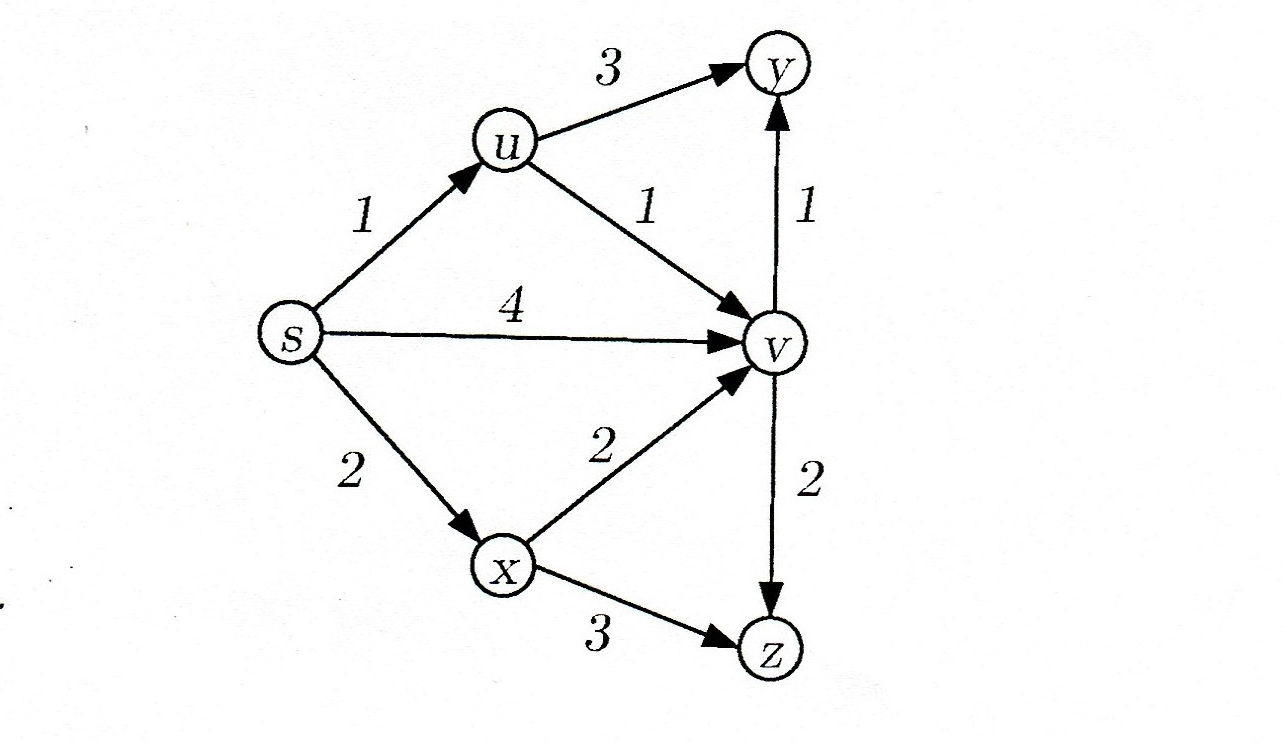
\includegraphics[scale=0.25]{./pictures/00_Graph}}
	\only<2> {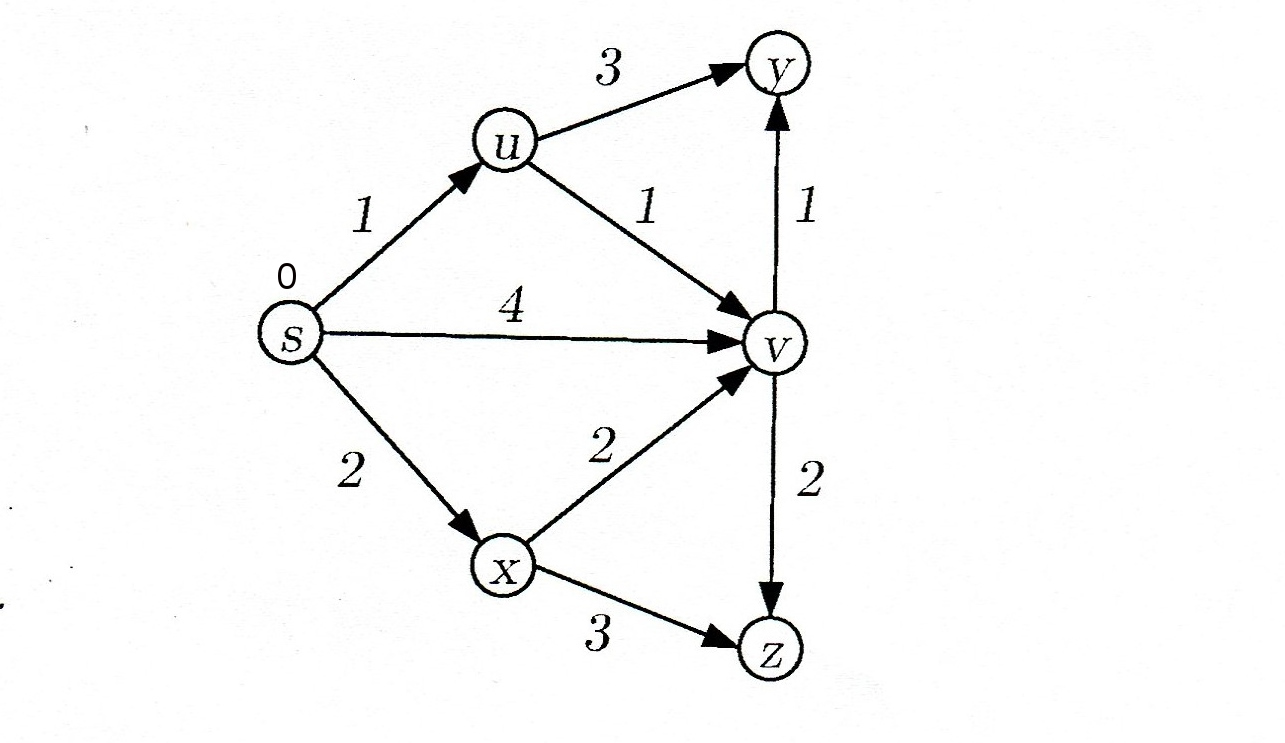
\includegraphics[scale=0.25]{./pictures/01_Graph}}
	\only<3> {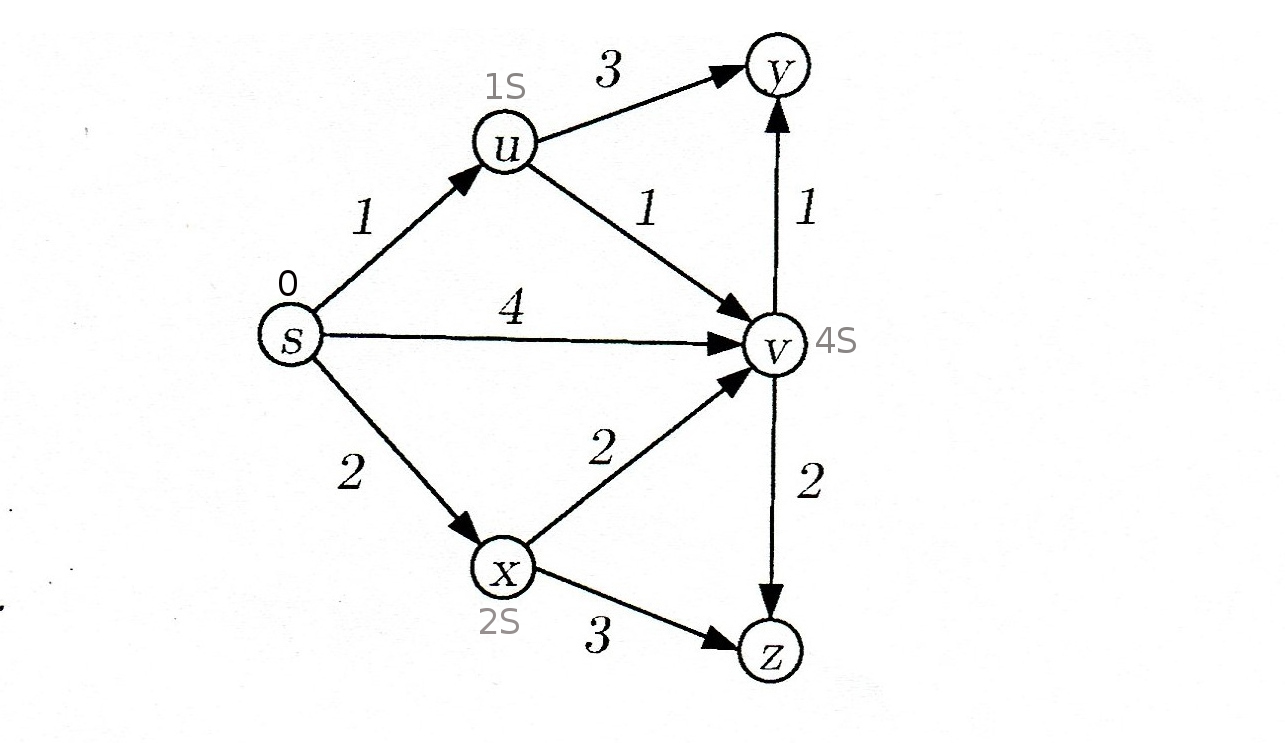
\includegraphics[scale=0.25]{./pictures/02_Graph}}
	\only<4> {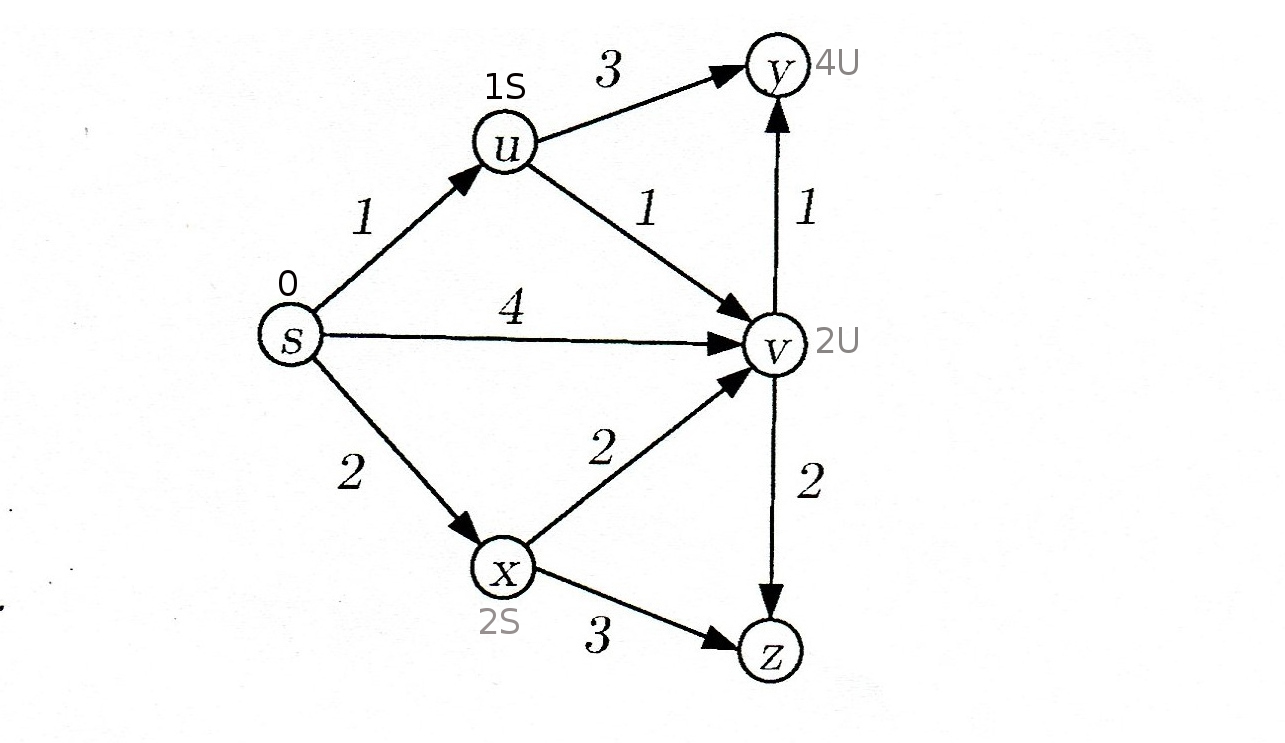
\includegraphics[scale=0.25]{./pictures/03_Graph}}
	\only<5> {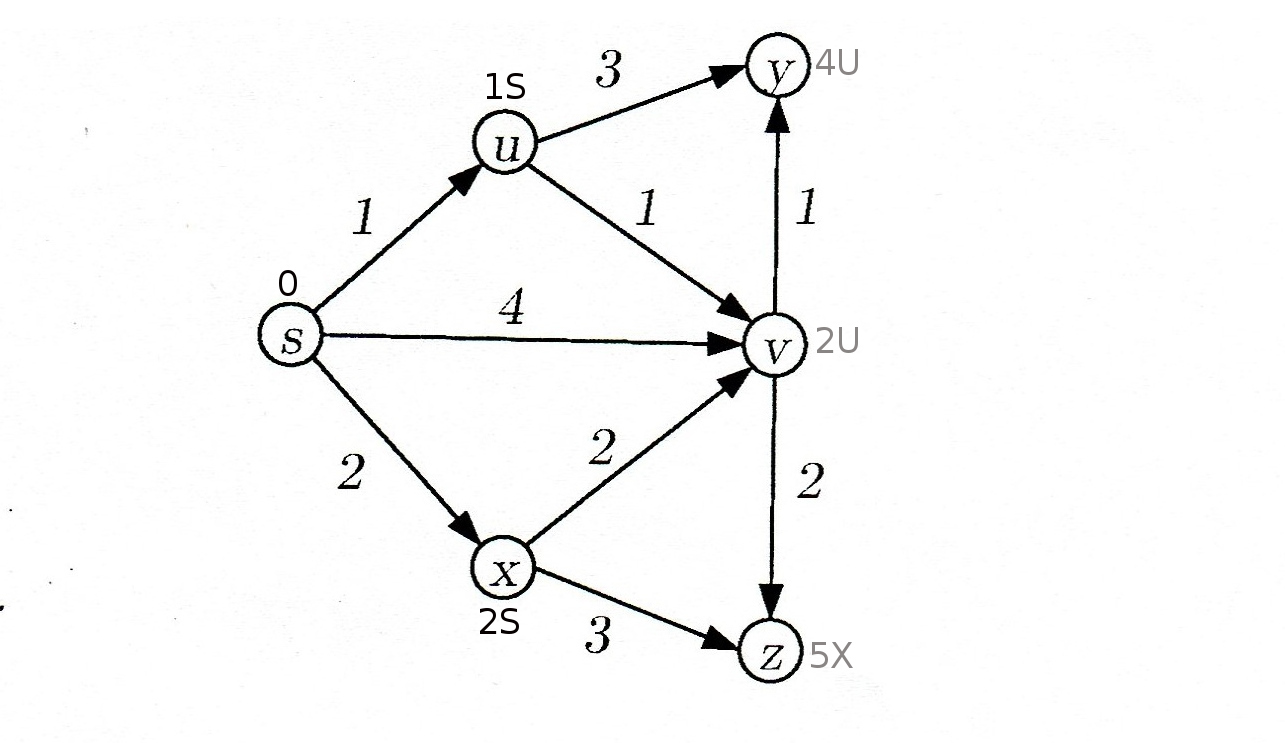
\includegraphics[scale=0.25]{./pictures/04_Graph}}
\end{frame}


\section{Komplexität}
\begin{frame}
	\begin{center}
		\LARGE {\textbf{Komplexität}}
	\end{center}
\end{frame}

\begin{frame}
	\begin{block} <1-> {Ursprüngliche Implementierung}
		\begin{itemize}
			\item <2--> Einzelschritte:
			\begin{itemize}
				\item <3-> Initialisieren der Arrays je $O(m)$
				\item <4-> Abarbeiten der grauen Knoten $O(m)$
				\item <5-> Bestimmen des Minimums $O(m)$
				\item <6-> Aktualisieren der Nachfolger $O(deg(v))$ \rightarrow $O(k)$
			\end{itemize}
			\item <7-> insgesamt Komplexität $O(m^{2})$
		\end{itemize}
	\end{block}	
\end{frame}

\begin{frame}
	\begin{block} <1-> {Implementierung mit Heap}
		\begin{itemize}
			\item <1-> Vorteile:
			\begin{itemize}
				\item <2-> Heapoperationen in $O(log m)$
				\item <3-> Bestimmen des Minimums in $O(log m)$
			\end{itemize}
			\item <4-> insgesamt Komplexität $O(k*log m)$
		\end{itemize}
	\end{block}		
\end{frame}

\section{Implementierung}
\begin{frame}
	\begin{block} <1-> {Eigenschaften}
		\begin{itemize}
			\item <2-> Programmiersprache: Python
			\item <3-> Umsetzung mit Heap (Priority Queue)
			\item <4-> keine Speicherung der Farbstufen wie bei Dijkstra
				\begin{itemize}
					\item <5-> kürzerer und übersichtlicherer Code
				\end{itemize}
		\end{itemize}
	\end{block}	
\end{frame}


\begin{frame}
\frametitle{Kompletter Code}
\lstset{language=Python}
\begin{lstlisting}
from heapq import heappush, heappop

def dijkstra_pq(G,s):
    m = len(G)                              #O(1)
    pq = []       #priority queue           #O(1)
    d = [None]*m  #kosten                   #O(m)
    p = [None]*m  #vorgaenger		       #O(m)
    d[s] = 0                                #O(1)
    heappush(pq, (0,s))                     #O(log m)
    while pq:                               #O(m)
        (_,v) = heappop(pq)                 #O(log m)
        for u in G[v]:                      #O(deg(v)) --> O(k)  
            alt = d[v] + G[v][u]            #O(1)
            if d[u]== None or alt < d[u]:   #O(1)
                d[u] = alt		            #O(1)	
               	p[u] = v                    #O(1)
                heappush(pq, (alt,u))       #O(log m)        
    return d,p

def shortest_path(s,v,p):
	if v == None:
		return []
	else:
		return shortest_path(s,p[v],p) + [v]
 
#Graph: 
    
def define_G():
    G = [   {1:1, 4:4, 2:2},   # Nachfolger von s
            {3:3, 4:1},        # von u
            {4:2, 5:3},        # von x
            {},                # von y
            {3:1, 5:2},        # von v
            {}                 # von z
        ]
    return G


G = define_G()
d,p = dijkstra_pq(G,0)
print( shortest_path(0,5,p))
print( shortest_path(0,3,p))
\end{lstlisting}
\end{frame}


\begin{frame}
	\begin{block} <1-> {Eingabe}
		\begin{itemize}
	
		\end{itemize}
	\end{block}	
\end{frame}


\begin{frame}
	\begin{block} <1-> {Algorithmus}
		\begin{itemize}
		\item <1-> Initialisierung
		\item <2-> Erweitern
		\item <3-> Aktualisieren
		\end{itemize}
	\end{block}	
\end{frame}


\begin{frame}
	\begin{block} <1-> {Rekursives Bestimmen des Pfades}
		\begin{itemize}

		\end{itemize}
	\end{block}	
\end{frame}


\begin{frame}
	\begin{block} <1-> {Aufruf}
		\begin{itemize}

		\end{itemize}
	\end{block}	
\end{frame}


			




\end{document}
